\section{Calibrating cameras on the NAPLab car}

To accurately map objects perceived with individual camera to other camera frames or the real world, the cameras on the NAPLab car needed to be calibrated. Using NVIDIA DriveWorks \cite{driveworks-camera-calibration} we performed calibration of the cameras with respect to the car while it was stationary. This is known as static calibration, and the parameters for calibration includes the intrinsic model and the extrinsic orientation and position. The intrinsic model calculates the geometrical relationship between pixels and optical rays for a camera, while the extrinsic model calculates the orientation and position in relation to the car. The two models are shown in \cref{fig:intrinsic-vs-extrinsic-calibration}.

\begin{figure}[htbp]
    \centering
    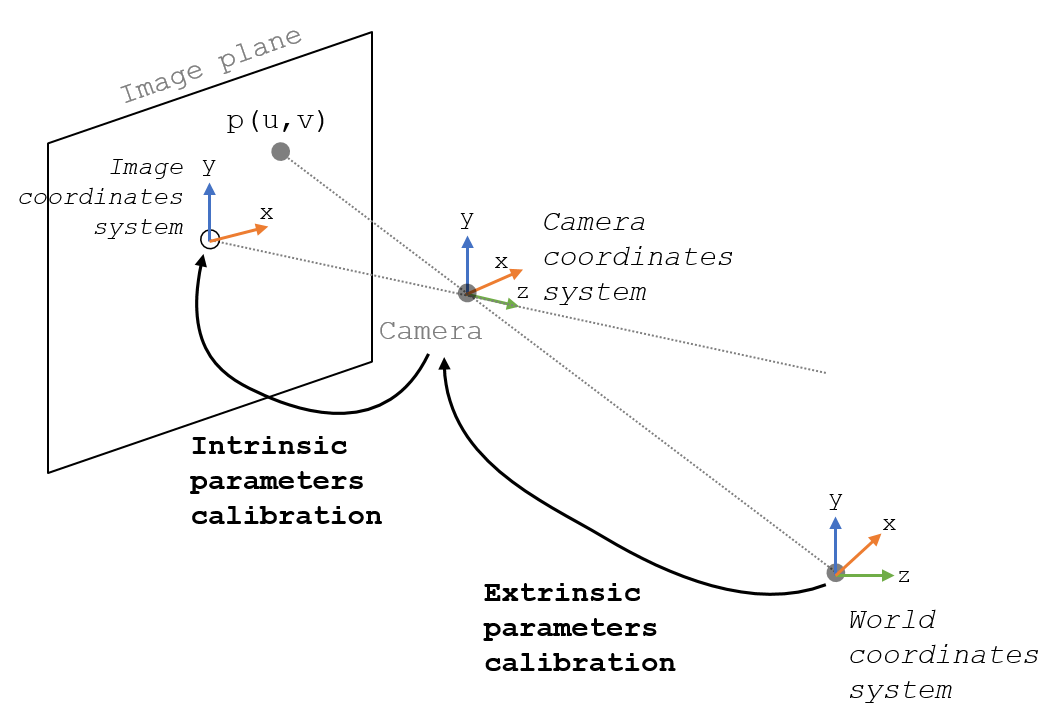
\includegraphics[width=0.7\textwidth]{chapters/3-method/figures/calibration/intrinsic-vs-extrinsic.png}
    \caption{Intrinsic vs. extrinsic parameters calibration. Source: \cite{intrinsic-vs-extrinsic-calibration}.}
    \label{fig:intrinsic-vs-extrinsic-calibration}
\end{figure}


\cref{fig:calibration-intrinsics,fig:calibration-extrinsics} show and describe the calibration process in more detail. While the intrinsic data was captured by the mounted cameras only, the extrinsic data had to be captured both from the mounted cameras and an external camera.

\todo[inline]{describe received rigfile}

 
\begin{figure}[htbp]
    \centering
    
    \begin{subfigure}[htbp]{0.6\textwidth}
        \centering
        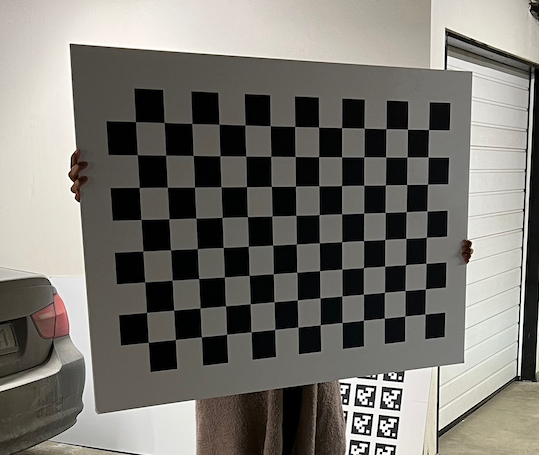
\includegraphics[width=\textwidth]{chapters/3-method/figures/calibration/checkerboard.jpeg}
        \caption{Checkerboard used for intrinsic camera calibration.}
    \end{subfigure}

    \bigskip

    \begin{subfigure}[htbp]{\textwidth}
        \centering
        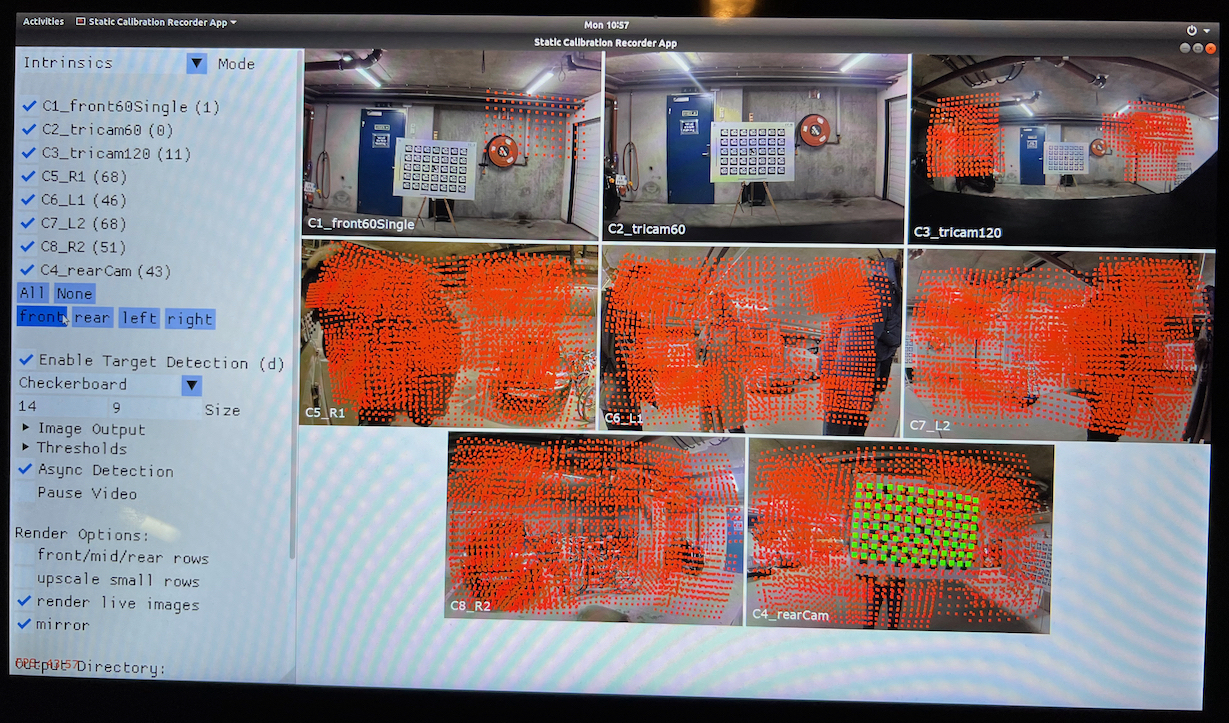
\includegraphics[width=\textwidth]{chapters/3-method/figures/calibration/intrinsics.jpeg}
        \caption{Software used for intrinsic camera calibration.}
    \end{subfigure}
    
    \caption{To perform intrinsic camera calibration, we moved a checkerboard across the camera view both vertically and horizontally until it had covered the whole view. We additionally rotated the checkerboard and moved it closer and further away from the camera to calibrate rotation and scale. This was repeated for all cameras. The DriveWorks software \cite{driveworks-camera-calibration} assisted in making sure we covered the whole area. The red dots are snapshots of the checkerboard, while the green dots show the current location of the checkerboard.}
    \label{fig:calibration-intrinsics}
\end{figure}


 \begin{figure}[htbp]
    \centering
    
    \begin{subfigure}[htbp]{\textwidth}
        \centering
        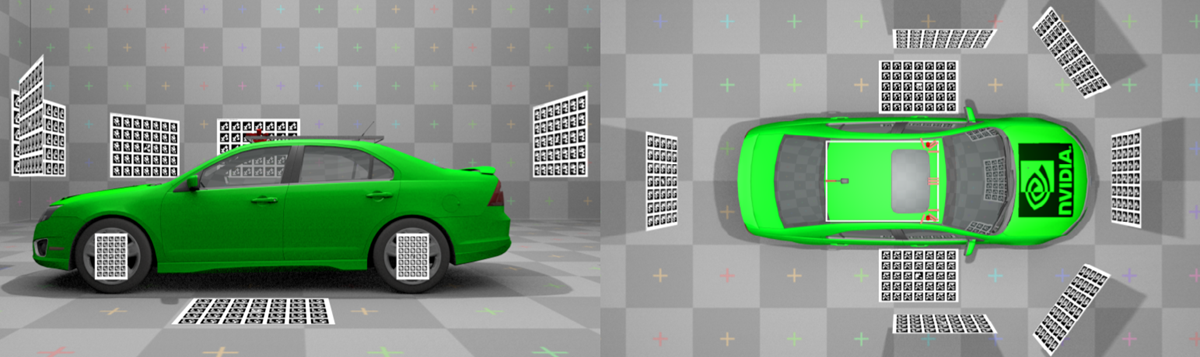
\includegraphics[width=\textwidth]{chapters/3-method/figures/calibration/nvidia-target-placement.png}
        \caption{Ideal target placement according to NVIDIA. Source: \cite{nvidia-drive-sim}.}
    \end{subfigure}

    \bigskip

    \begin{subfigure}[htbp]{\textwidth}
        \centering
        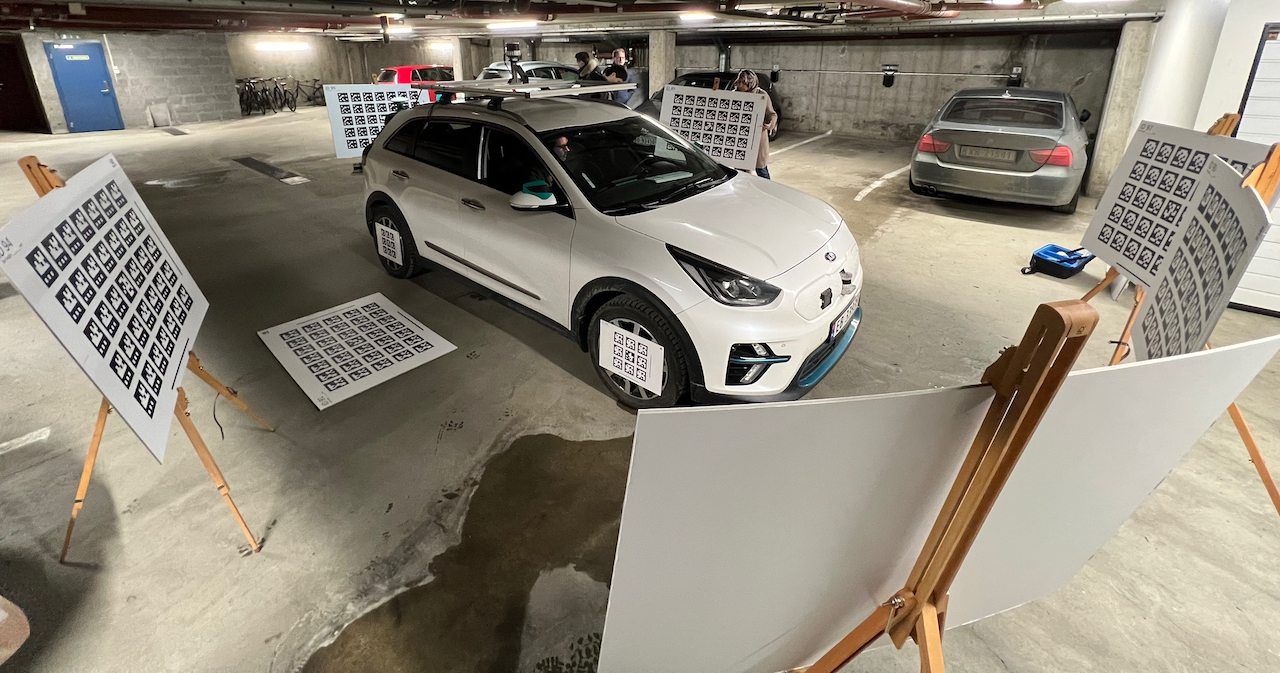
\includegraphics[width=\textwidth]{chapters/3-method/figures/calibration/extrinsics.jpeg}
        \caption{Our target placement around the NAPLab car.}
    \end{subfigure}
 
    \caption{To calibrate extrinsics, we placed eight large targets around the car and four small targets on the wheels. Each camera had to observe at least one large target. In addition to capturing images from the mounter cameras, a set of images also had to be captured by an external camera. These were used to create a link between targets that the cameras on the car itself could not observe.}
    \label{fig:calibration-extrinsics}
\end{figure}
